\textbf{RPG Game Database Design}

Version 1

Ahmad Abdel Razak Hussein Alkaseb Benjamin Sebastian Barrales Hernandez
Jeppe Ronning Koch Laith Abdel Razak Hussein Alkaseb Sadek Alsukafi

\begin{center}\rule{0.5\linewidth}{0.5pt}\end{center}

\begin{longtable}[]{@{}ll@{}}
\toprule
\textbf{Course} & Database \\
\midrule
\endhead
\textbf{Project} & RPG Game by Bajls \\
\textbf{Date of delivery} & 8/3/2026 \\
\textbf{List of figures} & 9 \\
\textbf{List of appendices} & 17 \\
\textbf{Number of characters (including spaces)} & 50939 \\
\bottomrule
\end{longtable}

\vspace{0.5cm}
\begin{center}
\begin{tabular}{ccc}
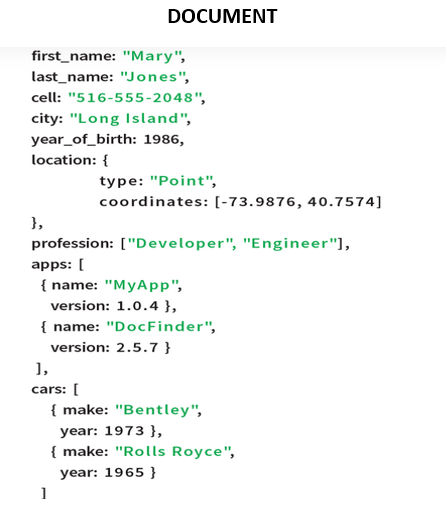
\includegraphics[width=0.30\textwidth,height=0.17\textheight,keepaspectratio]{images/frontpage/Document3.png} &
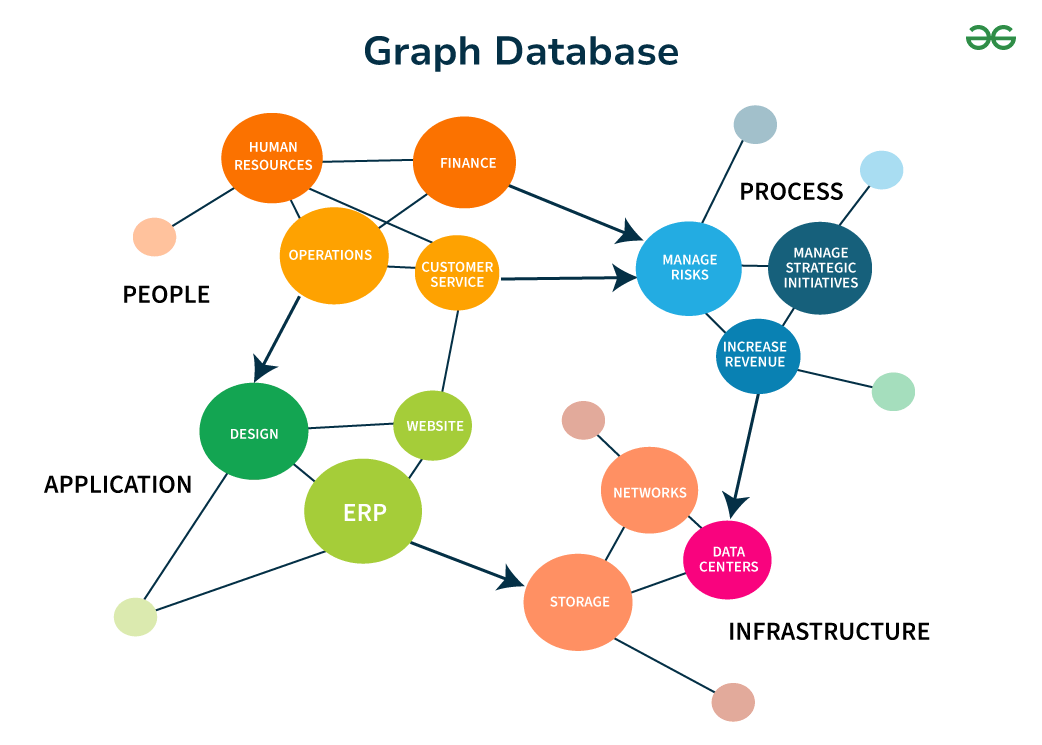
\includegraphics[width=0.30\textwidth,height=0.17\textheight,keepaspectratio]{images/frontpage/Graph-Database.png} &
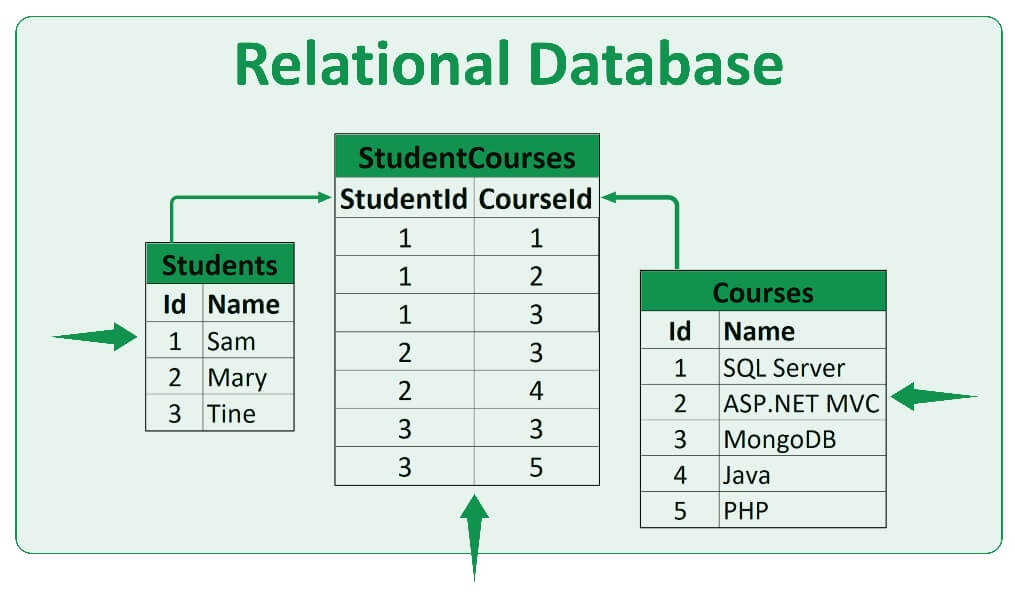
\includegraphics[width=0.30\textwidth,height=0.17\textheight,keepaspectratio]{images/frontpage/what-is-a-relational-database.jpg}
\end{tabular}
\end{center}

\thispagestyle{empty}

\newpage

\tableofcontents

\newpage

\hypertarget{introduction}{%
\section{1. Introduction}\label{introduction}}

Our goal is to design and develop a next-generation RPG game inspired by
the creative freedom and social interaction found in platforms like
Roblox. The game allows players to explore an interactive world,
customize their characters in detail, and engage in dynamic gameplay
experiences.

At its core, the game revolves around a customizable character that can
move freely in a large open world. Players experience the game through
their character, whose appearance, identity, and status are visible to
others in real time. As in Roblox-inspired games, visual identity and
personalization are central to the player experience.

The first development phase focuses on character customization and
player identity. Players create a personal profile and design one or
more unique characters with specific physical traits and attributes.
These traits define how the character looks and can later support social
interactions and additional gameplay mechanics.

The world is structured around exploration, housing, and social systems
such as gangs. Every character is stored in a structured database that
maintains logical relationships between profiles, characters, roles, and
properties. The system enforces clear rules for ownership, identity, and
mandatory attributes.

The player experience includes:

\begin{itemize}
\tightlist
\item
  Creating a personal profile
\item
  Customizing characters with physical traits
\item
  Exploring the map
\item
  Owning a house
\item
  Optionally joining a gang
\item
  Interacting with other players
\end{itemize}

The game architecture must support both regular players and
administrators who manage the system.

\newpage

\hypertarget{system-overview-and-cloud-architecture}{%
\subsection{1.1. System overview and cloud
architecture}\label{system-overview-and-cloud-architecture}}

This project is organized as a Java application with a PostgreSQL
database. The same logical architecture is used in cloud deployment and
in local development, while runtime setup differs by environment.

\hypertarget{architecture-diagram-cloud-deployment}{%
\subsubsection{Architecture diagram (cloud
deployment)}\label{architecture-diagram-cloud-deployment}}

\begin{verbatim}
[Client / Browser / API Consumer]
                |
                v
       [Java Application Service]
         (REST + business logic)
                |
                v
         [PostgreSQL Database]
                |
                v
     [Persistent Cloud Volume/Storage]
\end{verbatim}

In cloud environments, the application service and database run as
separate managed workloads. The database persists data on dedicated
storage, while the application scales independently.

\hypertarget{local-development-deployment-docker-compose}{%
\subsubsection{\texorpdfstring{Local development deployment
(\texttt{docker-compose})}{Local development deployment (docker-compose)}}\label{local-development-deployment-docker-compose}}

The local setup uses \texttt{docker-compose.yml} in the project root to
start application and database services in one command.

\begin{verbatim}
docker-compose.yml
    |
    +-- service: app (Java 17 + Maven/Hibernate)
    |       |
    |       +-- depends_on: db
    |
    +-- service: db (PostgreSQL)
            |
            +-- volume: local persistent data
\end{verbatim}

Typical local startup command:

\begin{Shaded}
\begin{Highlighting}[]
\ExtensionTok{docker}\NormalTok{ compose up }\AttributeTok{{-}d}
\end{Highlighting}
\end{Shaded}

\newpage

\hypertarget{explanation-of-choices-for-databases-and-programming-languages-and-other-tools}{%
\subsection{1.2. Explanation of choices for databases and programming
languages, and other
tools}\label{explanation-of-choices-for-databases-and-programming-languages-and-other-tools}}

The project uses \textbf{PostgreSQL}\footnote{PostgreSQL Documentation:
  https://www.postgresql.org/docs/} as the database system because the
domain is strongly relational and depends on strict integrity rules.
PostgreSQL gives stable transactional behavior, strong foreign-key
enforcement, and good support for normalized schemas with junction
tables such as \texttt{gang\_affiliations}.

The application is implemented in \textbf{Java 17}\footnote{Java 17
  Documentation (Oracle): https://docs.oracle.com/en/java/javase/17/}
with \textbf{Maven}\footnote{Apache Maven Documentation:
  https://maven.apache.org/guides/} as the build tool. Java was selected
because the project team works with an object-oriented domain model, and
Java integrates directly with JPA annotations for entity mapping. Maven
provides predictable dependency management and reproducible builds
across environments.

For persistence, the project uses \textbf{Hibernate (JPA)}\footnote{Hibernate
  ORM Documentation: https://hibernate.org/orm/documentation/}. This
allows the team to model business entities (\texttt{Profile},
\texttt{GameCharacter}, \texttt{House}, \texttt{Gang}, \texttt{Role},
\texttt{Gender}, \texttt{Weight}, \texttt{Height}, \texttt{EyeColor},
\texttt{SkinColor}) directly in code and keep the SQL schema aligned
through mapping metadata. Hibernate is configured for PostgreSQL and
supports both local development and deployment profiles through
environment variables.

Additional tools include:

\begin{itemize}
\tightlist
\item
  \textbf{Lombok} for reducing boilerplate code in entities (getters,
  setters, constructors, builders).
\item
  \textbf{Testcontainers} for disposable PostgreSQL instances during
  tests, which improves repeatability and reduces local setup variance.
\item
  \textbf{pgAdmin} for visual inspection of the physical schema and
  foreign key network.
\end{itemize}

The next chapter turns these technology choices into concrete database
rules and schema decisions.

\begin{center}\rule{0.5\linewidth}{0.5pt}\end{center}

\newpage

\hypertarget{relational-database}{%
\section{2. Relational database}\label{relational-database}}

This section defines the functional requirements for our RPG game
inspired by Roblox. The purpose is to clearly define persons, profiles,
characters, and their relationships in the system. The system must
enforce strict rules to ensure data integrity, logical consistency, and
reliable gameplay functionality.

To keep a clear thread through the chapter, we move in this order:
requirements -\textgreater{} conceptual/logical design -\textgreater{}
normalization -\textgreater{} physical implementation -\textgreater{}
stored database objects -\textgreater{} realistic seed data
-\textgreater{} access control.

\hypertarget{intro-to-relational-databases}{%
\subsection{2.1. Intro to relational
databases}\label{intro-to-relational-databases}}

A relational database organizes information in tables connected by keys.
This model is suitable for the RPG domain because core business rules
are relationship-based: one profile can own many characters, each
character must belong to exactly one profile, and gang membership is
many-to-many through a junction table.

Relational systems are also appropriate when consistency is more
important than schema flexibility. In this project, invalid states such
as characters without profiles, houses without owners, or duplicate
membership records must be prevented in the database itself. PostgreSQL
handles this through primary keys, foreign keys, unique constraints, and
transaction guarantees.

\hypertarget{database-design}{%
\subsection{2.2. Database design}\label{database-design}}

The database design follows a layered progression from requirements to
implementation:

\begin{itemize}
\tightlist
\item
  First, domain requirements define mandatory entities.
\item
  Next, the conceptual and logical models translate those rules into
  normalized relations.
\item
  Finally, the physical model implements data types, keys, and
  constraints in PostgreSQL/Hibernate.
\end{itemize}

This process ensures that design decisions are traceable from business
rules to concrete table definitions and mapping annotations.

\newpage

\hypertarget{profile-and-role-requirements}{%
\subsubsection{Profile and Role
Requirements}\label{profile-and-role-requirements}}

\hypertarget{person-and-profile}{%
\paragraph{Person and Profile}\label{person-and-profile}}

\begin{itemize}
\tightlist
\item
  A person can have exactly one profile in the system.
\item
  The profile represents the player's digital identity.
\item
  A profile must be uniquely identifiable (for example by
  \texttt{profile\_id} or \texttt{username}).
\item
  A person is not allowed to create multiple profiles.
\end{itemize}

This ensures that each real-world player is connected to one controlled
game identity.

\hypertarget{role-system}{%
\paragraph{Role System}\label{role-system}}

\begin{itemize}
\tightlist
\item
  A profile must have exactly one role.
\item
  The role can be either \texttt{User} or \texttt{Admin}.
\item
  A profile cannot have multiple roles at the same time.
\item
  \texttt{Admin} accounts have extended permissions compared to
  \texttt{User} accounts, such as management and moderation
  functionality.
\end{itemize}

This establishes role-based access control in the game.

\hypertarget{character-requirements}{%
\subsubsection{Character Requirements}\label{character-requirements}}

\hypertarget{profile-to-character-relationship}{%
\paragraph{Profile to Character
Relationship}\label{profile-to-character-relationship}}

\begin{itemize}
\tightlist
\item
  A profile can have one or more characters.
\item
  A character must belong to exactly one profile.
\item
  A character cannot exist without being linked to a profile.
\end{itemize}

This creates a one-to-many relationship between \texttt{Profile} and
\texttt{Character}.

\hypertarget{character-attributes}{%
\paragraph{Character Attributes}\label{character-attributes}}

Each character must have exactly one of each required attribute:

\begin{itemize}
\tightlist
\item
  One gender
\item
  One weight
\item
  One height
\item
  One eye color
\item
  One skin color
\end{itemize}

All attributes are mandatory and cannot be empty. A character cannot
have multiple values for any of these attributes. The system must
validate that all required attributes are present before a character can
be created.

\newpage

\hypertarget{housing-requirement}{%
\paragraph{Housing Requirement}\label{housing-requirement}}

\begin{itemize}
\tightlist
\item
  A character must have exactly one house.
\item
  A character cannot exist without an assigned house.
\item
  A house belongs to exactly one character.
\item
  A house cannot be shared by multiple characters.
\end{itemize}

This creates a mandatory one-to-one relationship between
\texttt{Character} and \texttt{House}. The system must prevent
characters without houses and houses without assigned characters.

\hypertarget{gang-membership-requirement}{%
\paragraph{Gang Membership
Requirement}\label{gang-membership-requirement}}

\begin{itemize}
\tightlist
\item
  Gang membership is optional.
\item
  A character can belong to zero or more gangs.
\item
  A gang can have zero or more characters.
\end{itemize}

This establishes an optional many-to-many relationship between
\texttt{Character} and \texttt{Gang}.

\hypertarget{data-integrity-rules}{%
\paragraph{Data Integrity Rules}\label{data-integrity-rules}}

The system must enforce the following constraints:

\begin{itemize}
\tightlist
\item
  Every person has at most one profile.
\item
  Every profile has exactly one role.
\item
  Every character belongs to exactly one profile.
\item
  Every character has all required physical attributes.
\item
  Every character has exactly one house.
\item
  A character may belong to zero or more gangs.
\end{itemize}

The system must prevent invalid states such as orphan characters,
missing houses, missing roles, or duplicate role assignments.

\hypertarget{relationship-summary}{%
\paragraph{Relationship Summary}\label{relationship-summary}}

\begin{itemize}
\tightlist
\item
  \texttt{Profile} to \texttt{Role}: Many-to-One
\item
  \texttt{Profile} to \texttt{Character}: One-to-Many
\item
  \texttt{Character} to \texttt{House}: One-to-One (Mandatory)
\item
  \texttt{Character} to \texttt{Gang}: Optional Many-to-Many
\item
  \texttt{Character} to Attributes: Many-to-One
\end{itemize}

\hypertarget{conclusion}{%
\paragraph{Conclusion}\label{conclusion}}

These requirements define the structural foundation of the RPG system.
They ensure clear identity management, controlled permissions, complete
character definitions, and mandatory housing ownership. This
specification forms the basis for conceptual, logical, and physical
database modeling.

\begin{center}\rule{0.5\linewidth}{0.5pt}\end{center}

\newpage

\hypertarget{entityrelationship-model-conceptual---logical---physical-model}{%
\subsubsection{2.2.1. Entity/Relationship Model (Conceptual
-\textgreater{} Logical -\textgreater{} Physical
model)}\label{entityrelationship-model-conceptual---logical---physical-model}}

This section presents the entity/relationship progression from
conceptual understanding to logical structure, and prepares the
transition to the physical implementation in Section 2.3.

\hypertarget{conceptual-model}{%
\paragraph{Conceptual Model}\label{conceptual-model}}

The conceptual model describes the business domain without technical
implementation details such as data types, indexes, or SQL syntax. Its
purpose is to show what information the system must manage and how core
concepts are related from a game and business perspective. In this
project, \texttt{Characters} is the central concept because most game
actions, ownership rules, and social interactions are represented
through character entities.

\hypertarget{conceptual-diagram}{%
\paragraph{Conceptual Diagram}\label{conceptual-diagram}}

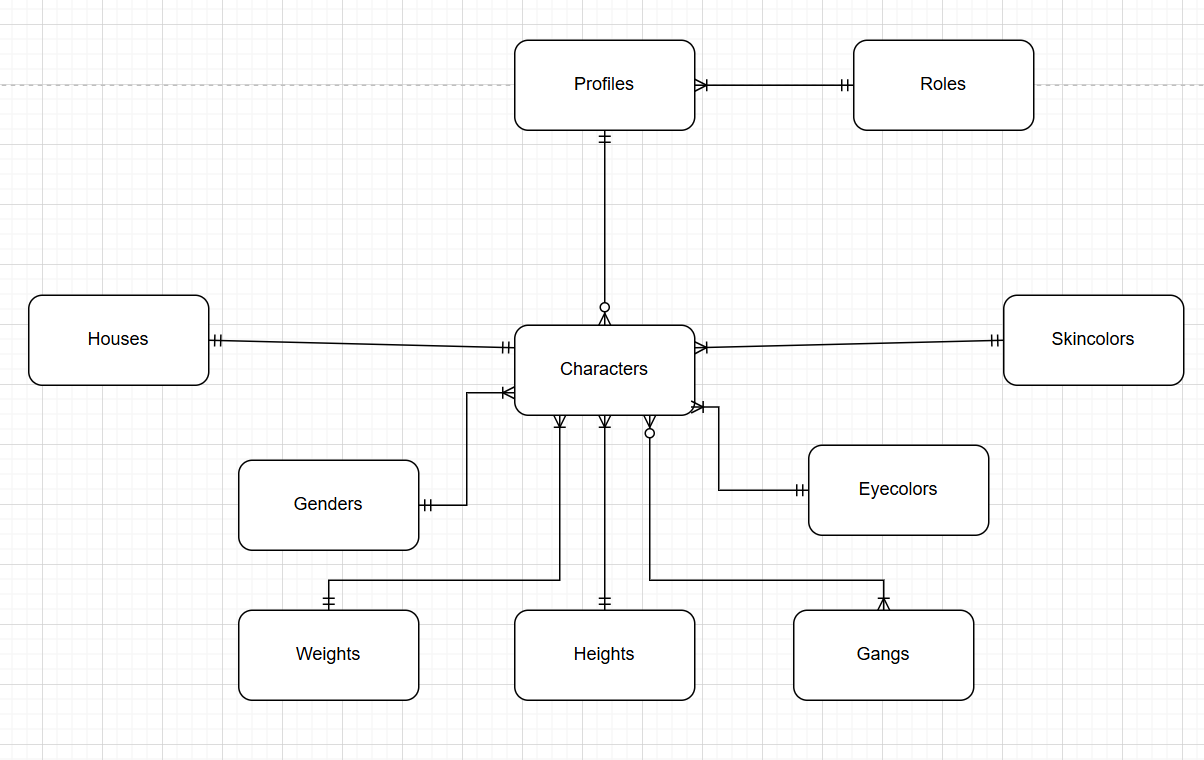
\includegraphics{images/conceptual-logical-physical/conceptual-model-2026-02-10.png}
\emph{Date: 10.2.2026}

The model includes the following core entities:

\begin{itemize}
\tightlist
\item
  \textbf{Profiles}: the persistent player identity used for login and
  account-level ownership.
\item
  \textbf{Roles}: access-level definitions (\texttt{User} and
  \texttt{Admin}) connected to profile permissions.
\item
  \textbf{Characters}: playable identities controlled by profiles inside
  the game world.
\item
  \textbf{Houses}: character-owned properties used to represent private
  assets and ownership constraints.
\item
  \textbf{Gangs}: social groups that support optional membership and
  multi-character affiliation.
\item
  \textbf{Genders, Weights, Heights, Eyecolors, Skincolors}: controlled
  attribute domains used to define mandatory character appearance
  traits.
\end{itemize}

\newpage

\hypertarget{key-relationships-in-the-diagram}{%
\paragraph{Key Relationships in the
Diagram}\label{key-relationships-in-the-diagram}}

\begin{itemize}
\tightlist
\item
  \texttt{Profiles} to \texttt{Roles}: many-to-one. Each profile has
  exactly one role, while one role can be assigned to many profiles.
\item
  \texttt{Profiles} to \texttt{Characters}: one-to-many. A profile can
  own multiple characters, and each character belongs to one profile.
\item
  \texttt{Characters} to \texttt{Houses}: one-to-one (mandatory). Each
  character must be linked to one house, and each house belongs to one
  character.
\item
  \texttt{Characters} to appearance tables (\texttt{Genders},
  \texttt{Weights}, \texttt{Heights}, \texttt{Eyecolors},
  \texttt{Skincolors}): many-to-one for each attribute. Each character
  has exactly one value per attribute, and many characters can share the
  same attribute value.
\item
  \texttt{Characters} to \texttt{Gangs}: optional many-to-many. A
  character may join zero or more gangs, and each gang may contain
  multiple characters.
\end{itemize}

\hypertarget{cardinality-and-modality}{%
\paragraph{Cardinality and Modality}\label{cardinality-and-modality}}

In this project, relationship rules are described using both
\textbf{cardinality} and \textbf{modality}:

\begin{itemize}
\tightlist
\item
  \textbf{Cardinality} defines the maximum number of related rows (for
  example one-to-one, one-to-many, many-to-many).
\item
  \textbf{Modality} defines whether participation is mandatory or
  optional (minimum 1 or minimum 0).
\end{itemize}

Applied to our model:

\begin{itemize}
\tightlist
\item
  \texttt{Profile} -\textgreater{} \texttt{Character}: cardinality is
  one-to-many, modality is mandatory on \texttt{Character} side (every
  character must have one profile) and optional on profile side (a
  profile can exist with zero characters).
\item
  \texttt{Character} -\textgreater{} \texttt{House}: cardinality is
  one-to-one, modality is mandatory on character side in our JPA mapping
  because \texttt{characters.house\_id} is \texttt{NOT\ NULL} and
  \texttt{UNIQUE}. On house side, a house can exist without being
  referenced by a character unless extra business rules are added.
\item
  \texttt{Character} \textless-\textgreater{} \texttt{Gang}: cardinality
  is many-to-many via \texttt{gang\_affiliations}, modality is optional
  on both sides (0..N).
\item
  \texttt{Character} -\textgreater{} attribute reference tables
  (\texttt{Gender}, \texttt{Weight}, \texttt{Height}, \texttt{EyeColor},
  \texttt{SkinColor}): cardinality is many-to-one, modality is mandatory
  on character side because each FK is required.
\end{itemize}

The conceptual model also defines participation rules. Participation is
mandatory for \texttt{Character} to \texttt{Profile}, \texttt{Character}
to \texttt{House}, and \texttt{Character} to each appearance category
because these are required for valid gameplay state. Participation is
optional for gang membership because not all players must engage in
group-based social mechanics.

From a domain perspective, this model prevents ambiguous ownership. A
profile owns characters, characters own houses, and social membership is
kept independent through gangs. This separation is important because
each area has different lifecycle rules: deleting or deactivating a
profile affects owned characters, while gang membership can be added or
removed without changing character identity.

The conceptual view therefore acts as the foundation for the next
models. It communicates business meaning to both technical and
non-technical stakeholders, verifies that rules are complete before
implementation, and reduces redesign risk later in the project.

\newpage

\hypertarget{logical-model}{%
\paragraph{Logical Model}\label{logical-model}}

The logical model translates the conceptual design into a normalized
relational structure. At this level business rules are transformed into
enforceable structural constraints with attributes.

\hypertarget{logical-diagram}{%
\paragraph{Logical Diagram}\label{logical-diagram}}

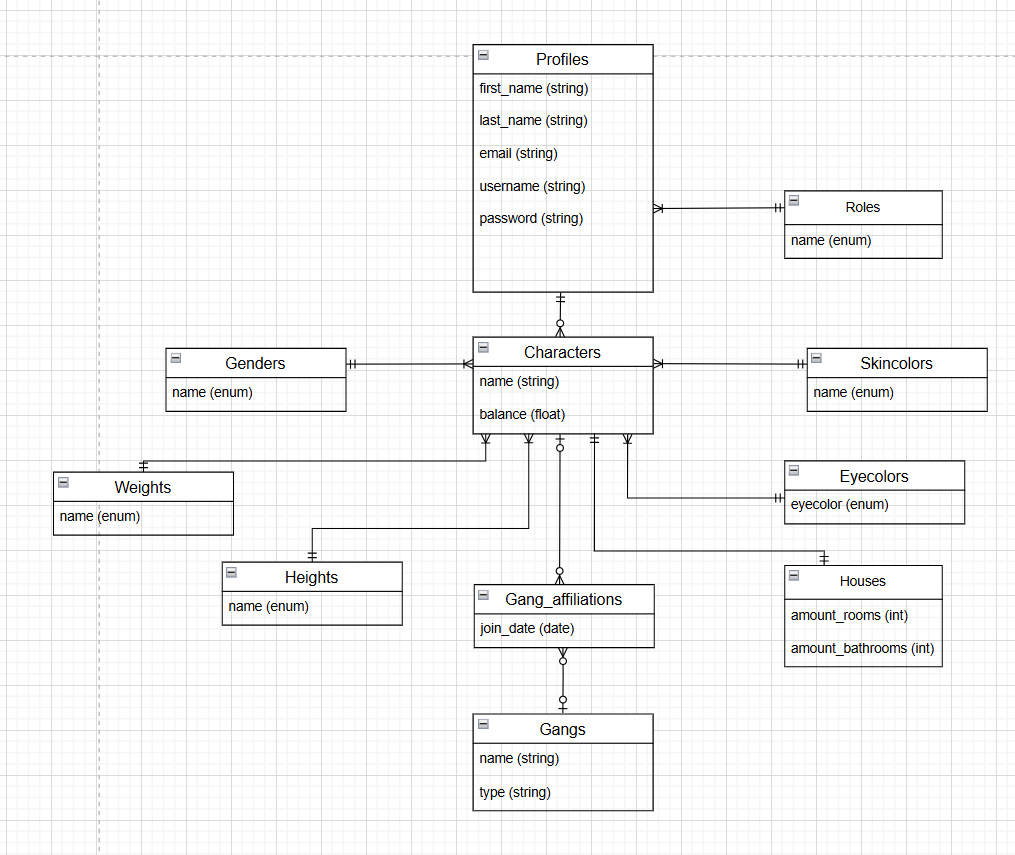
\includegraphics{images/conceptual-logical-physical/logical-model-2026-02-10.png}
\emph{Date: 10.2.2026}

\hypertarget{main-tables}{%
\paragraph{Main Tables}\label{main-tables}}

\begin{itemize}
\tightlist
\item
  \textbf{Profiles} (first\_name, last\_name, email, username, password)
\item
  \textbf{Roles} (name)
\item
  \textbf{Characters} (name, balance)
\item
  \textbf{Houses} (amount\_rooms, amount\_bathrooms)
\item
  \textbf{Gangs} (name, type)
\item
  \textbf{Gang\_Affiliations} (join\_date)
\item
  \textbf{Genders, Weights, Heights, Eyecolors, Skincolors} (name)
\end{itemize}

The table layout intentionally separates high-change data from
low-change reference data. \texttt{characters} is transaction-heavy and
contains gameplay-relevant state, while reference tables hold stable
classification values. This design reduces redundancy and makes updates
predictable. For example, changing a reference label does not require
editing every character row.

\hypertarget{logical-relationship-rules}{%
\paragraph{Logical Relationship
Rules}\label{logical-relationship-rules}}

\begin{itemize}
\tightlist
\item
  One \texttt{Profile} belongs to one \texttt{Role}; one \texttt{Role}
  can be used by many profiles.
\item
  One \texttt{Profile} can own many \texttt{Characters}.
\item
  Each \texttt{Character} must reference exactly one value in each
  attribute category.
\item
  \texttt{Character} and \texttt{House} are modeled as a mandatory
  one-to-one relationship.
\item
  \texttt{Character} and \texttt{Gang} are modeled through the junction
  table \texttt{Gang\_Affiliations} (many-to-many).
\end{itemize}

In addition to these cardinalities, the logical model defines key
strategy and uniqueness boundaries:

\begin{itemize}
\tightlist
\item
  \texttt{username} should be unique at profile level to guarantee a
  single login identity per player.
\end{itemize}

This structure keeps the data model clear and easier to maintain.
Relationships are defined in a simple way, so common queries are easier
to build and understand before implementing the final PostgreSQL
optimization.

\hypertarget{normalization-process}{%
\subsubsection{2.2.2. Normalization
process}\label{normalization-process}}

Normalization keeps data in one place and makes updates and queries more
consistent. The goal is to eliminate redundancy and avoid insertion,
update, and deletion anomalies that would otherwise appear in gameplay
data.

\hypertarget{first-normal-form-1nf}{%
\paragraph{First Normal Form (1NF)}\label{first-normal-form-1nf}}

1NF requires atomic attributes and no repeating groups in a single
column. In this schema, all tables satisfy 1NF because each column holds
one value per row. For example, a character does not store multiple eye
colors or multiple gang IDs in one field. Multi-valued relationships are
modeled through separate tables (especially
\texttt{gang\_affiliations}).

\hypertarget{second-normal-form-2nf}{%
\paragraph{Second Normal Form (2NF)}\label{second-normal-form-2nf}}

2NF requires that non-key attributes depend on the full primary key, not
part of it. This is especially relevant in tables with composite keys.
\texttt{gang\_affiliations} satisfies 2NF because \texttt{join\_date}
depends on the specific combination of \texttt{character\_id} and
\texttt{gang\_id} rather than only one of them. No partial dependency is
present.

\hypertarget{third-normal-form-3nf}{%
\paragraph{Third Normal Form (3NF)}\label{third-normal-form-3nf}}

3NF removes transitive dependencies where non-key attributes depend on
other non-key attributes. The schema satisfies this by separating roles,
appearance categories, and gangs into dedicated tables referenced by
foreign keys. For example, role names are not duplicated in
\texttt{profiles}, and appearance labels are not duplicated in
\texttt{characters}.

The resulting 3NF design improves consistency and maintainability:

\begin{itemize}
\tightlist
\item
  Changes are localized to one table.
\item
  Duplicate text values are minimized.
\item
  Integrity constraints become easier to enforce.
\item
  Queries stay clear and consistent as data grows.
\end{itemize}

The final logical schema therefore satisfies \textbf{3NF} and provides a
reliable base for physical implementation.

\begin{center}\rule{0.5\linewidth}{0.5pt}\end{center}

\newpage

\hypertarget{physical-data-model}{%
\subsection{2.3. Physical data model}\label{physical-data-model}}

\hypertarget{database-setup-and-schema-execution}{%
\paragraph{Database setup and schema
execution}\label{database-setup-and-schema-execution}}

The physical database can be created directly from
\texttt{sqls/schema.sql}. This makes onboarding simple: one script
builds the tables, keys, and constraints used by the project.

\hypertarget{schema-export}{%
\paragraph{Schema export}\label{schema-export}}

To make the database reproducible without access to the project host, a
full schema export is included as \texttt{sqls/schema.sql}. The file is
generated with \texttt{pg\_dump} and contains the DDL (Data Definition
Language) needed to recreate the database structure: tables,
constraints, foreign keys, indexes, and sequences.

The schema file acts as a portable snapshot of the physical data model.
Anyone cloning the repository can create an identical empty database by
running:

\begin{Shaded}
\begin{Highlighting}[]
\ExtensionTok{psql} \AttributeTok{{-}U}\NormalTok{ postgres }\AttributeTok{{-}d}\NormalTok{ bajls }\AttributeTok{{-}f}\NormalTok{ sqls/schema.sql}
\end{Highlighting}
\end{Shaded}

If your local database name is different, replace \texttt{bajls} with
your own database name (for example \texttt{bajls\_db}).

Minimum setup:

\begin{Shaded}
\begin{Highlighting}[]
\ExtensionTok{createdb}\NormalTok{ bajls\_db}
\ExtensionTok{psql} \AttributeTok{{-}d}\NormalTok{ bajls\_db }\AttributeTok{{-}f}\NormalTok{ sqls/schema.sql}
\end{Highlighting}
\end{Shaded}

Clean reset (useful during development):

\begin{Shaded}
\begin{Highlighting}[]
\ExtensionTok{dropdb} \AttributeTok{{-}{-}if{-}exists}\NormalTok{ bajls\_db}
\ExtensionTok{createdb}\NormalTok{ bajls\_db}
\ExtensionTok{psql} \AttributeTok{{-}d}\NormalTok{ bajls\_db }\AttributeTok{{-}f}\NormalTok{ sqls/schema.sql}
\end{Highlighting}
\end{Shaded}

If your PostgreSQL user is not the default user, specify it explicitly:

\begin{Shaded}
\begin{Highlighting}[]
\ExtensionTok{psql} \AttributeTok{{-}U}\NormalTok{ postgres }\AttributeTok{{-}d}\NormalTok{ bajls\_db }\AttributeTok{{-}f}\NormalTok{ sqls/schema.sql}
\end{Highlighting}
\end{Shaded}

\hypertarget{what-the-schema-script-creates}{%
\paragraph{What the schema script
creates}\label{what-the-schema-script-creates}}

The script creates the database structure in a logical order:

\begin{itemize}
\tightlist
\item
  Reference tables first (for controlled values), such as
  \texttt{roles}, \texttt{genders}, \texttt{weights}, \texttt{heights},
  \texttt{eyecolors}, and \texttt{skincolors}.
\item
  Core business tables next, such as \texttt{profiles},
  \texttt{characters}, \texttt{houses}, and \texttt{gangs}.
\item
  Relationship table last: \texttt{gang\_affiliations}, which links
  characters and gangs in a many-to-many pattern.
\end{itemize}

This order matters because foreign keys can only point to tables that
already exist.

\hypertarget{how-constraints-implement-business-rules}{%
\paragraph{How constraints implement business
rules}\label{how-constraints-implement-business-rules}}

Example from the same pattern used in \texttt{sqls/schema.sql}:

\begin{Shaded}
\begin{Highlighting}[]
\KeywordTok{CREATE} \KeywordTok{TABLE}\NormalTok{ characters (}
    \KeywordTok{id}\NormalTok{ SERIAL }\KeywordTok{PRIMARY} \KeywordTok{KEY}\NormalTok{,}
\NormalTok{    profile\_id }\DataTypeTok{INTEGER} \KeywordTok{NOT} \KeywordTok{NULL} \KeywordTok{REFERENCES}\NormalTok{ profiles(}\KeywordTok{id}\NormalTok{),}
\NormalTok{    house\_id }\DataTypeTok{INTEGER} \KeywordTok{NOT} \KeywordTok{NULL} \KeywordTok{UNIQUE} \KeywordTok{REFERENCES}\NormalTok{ houses(}\KeywordTok{id}\NormalTok{)}
\NormalTok{);}
\end{Highlighting}
\end{Shaded}

This simple definition enforces important rules at database level:

\begin{itemize}
\tightlist
\item
  \texttt{PRIMARY\ KEY} gives each character a stable identity.
\item
  \texttt{NOT\ NULL} makes profile and house assignment mandatory.
\item
  \texttt{REFERENCES} prevents invalid IDs that do not exist in parent
  tables.
\item
  \texttt{UNIQUE} on \texttt{house\_id} enforces one house per character
  (one-to-one).
\end{itemize}

Many-to-many membership is handled with a junction table:

\begin{Shaded}
\begin{Highlighting}[]
\KeywordTok{CREATE} \KeywordTok{TABLE}\NormalTok{ gang\_affiliations (}
\NormalTok{    character\_id }\DataTypeTok{INTEGER} \KeywordTok{REFERENCES}\NormalTok{ characters(}\KeywordTok{id}\NormalTok{),}
\NormalTok{    gang\_id }\DataTypeTok{INTEGER} \KeywordTok{REFERENCES}\NormalTok{ gangs(}\KeywordTok{id}\NormalTok{),}
\NormalTok{    join\_date }\DataTypeTok{DATE}\NormalTok{,}
    \KeywordTok{PRIMARY} \KeywordTok{KEY}\NormalTok{ (character\_id, gang\_id)}
\NormalTok{);}
\end{Highlighting}
\end{Shaded}

The composite primary key prevents duplicate memberships for the same
character-gang pair.

\hypertarget{quick-verification-after-running-the-script}{%
\paragraph{Quick verification after running the
script}\label{quick-verification-after-running-the-script}}

After importing \texttt{sqls/schema.sql}, a developer can run short
checks:

\begin{Shaded}
\begin{Highlighting}[]
\CommentTok{{-}{-} list created tables}
\NormalTok{\textbackslash{}dt}

\CommentTok{{-}{-} inspect columns and constraints}
\NormalTok{\textbackslash{}d characters}
\NormalTok{\textbackslash{}d gang\_affiliations}
\end{Highlighting}
\end{Shaded}

And a quick join test:

\begin{Shaded}
\begin{Highlighting}[]
\KeywordTok{SELECT}\NormalTok{ c.}\KeywordTok{id}\NormalTok{, p.username, h.}\KeywordTok{id} \KeywordTok{AS}\NormalTok{ house\_id}
\KeywordTok{FROM}\NormalTok{ characters c}
\KeywordTok{JOIN}\NormalTok{ profiles p }\KeywordTok{ON}\NormalTok{ p.}\KeywordTok{id} \OperatorTok{=}\NormalTok{ c.profile\_id}
\KeywordTok{JOIN}\NormalTok{ houses h }\KeywordTok{ON}\NormalTok{ h.}\KeywordTok{id} \OperatorTok{=}\NormalTok{ c.house\_id}
\KeywordTok{LIMIT} \DecValTok{5}\NormalTok{;}
\end{Highlighting}
\end{Shaded}

If these queries run successfully, the schema is loaded and core
relationships are working as expected.

The physical model is the concrete PostgreSQL implementation of the
logical schema. At this stage, abstract relations are converted into
actual database objects with column types, constraints, and execution
characteristics. The implementation shown in pgAdmin reflects the final
table structure and foreign-key network used by the project.

\hypertarget{physical-diagram}{%
\paragraph{Physical Diagram}\label{physical-diagram}}

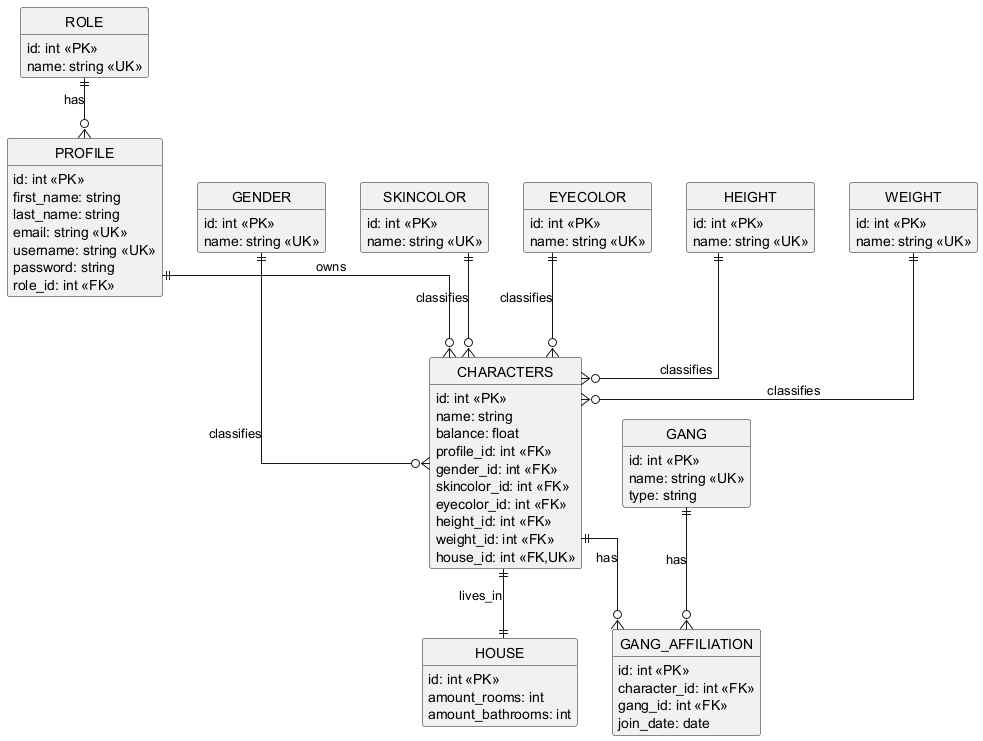
\includegraphics{images/conceptual-logical-physical/physical-model-2026-02-10.png}
\emph{Date: 10.2.2026}

\hypertarget{implementation-details}{%
\paragraph{Implementation Details}\label{implementation-details}}

\begin{itemize}
\tightlist
\item
  Primary keys are implemented as integer identifiers (\texttt{id}).
\item
  Foreign keys are created between dependent tables to enforce
  referential integrity.
\item
  The \texttt{characters.house\_id} column is unique, enforcing one
  house per character.
\item
  The \texttt{gang\_affiliations} table stores many-to-many links
  between characters and gangs, including \texttt{join\_date}.
\item
  Reference tables (\texttt{genders}, \texttt{weights},
  \texttt{heights}, \texttt{eyecolors}, \texttt{skincolors},
  \texttt{roles}) reduce redundancy and centralize valid values.
\end{itemize}

The PostgreSQL schema is designed to enforce business rules at database
level, not only in application code. Mandatory fields are protected with
\texttt{NOT\ NULL}, key relationships are protected with foreign keys,
and entity identity is protected with primary-key constraints. This
reduces the risk of inconsistent data even if multiple services or
scripts write to the same database.

For relationship-heavy queries, indexing strategy is important. Primary
keys are indexed automatically, and foreign-key columns should be
indexed to improve join performance, especially for frequent operations
such as loading profile characters, character attributes, or gang
memberships. As data volume increases, this prevents full-table scans
for common gameplay queries.

Operationally, the physical design also supports maintainability:

\begin{itemize}
\tightlist
\item
  Clear naming conventions for tables and columns.
\item
  Dedicated junction table for many-to-many associations.
\item
  Stable reference tables for controlled enumerations.
\item
  Predictable join paths for reporting and administration tools.
\end{itemize}

\hypertarget{cardinality-and-modality-in-the-physical-model}{%
\paragraph{Cardinality and Modality in the Physical
Model}\label{cardinality-and-modality-in-the-physical-model}}

At the physical level, cardinality and modality are enforced through
foreign keys, uniqueness, and nullability:

\begin{itemize}
\tightlist
\item
  \texttt{profiles.role\_id} is \texttt{NOT\ NULL} and references
  \texttt{roles.id}, so each profile must have exactly one role
  (mandatory many-to-one).
\item
  \texttt{characters.profile\_id} is \texttt{NOT\ NULL}, so each
  character must belong to one profile, while a profile can still have
  zero or many characters.
\item
  \texttt{characters.house\_id} is both \texttt{NOT\ NULL} and
  \texttt{UNIQUE}, enforcing one mandatory house per character and
  preventing multiple characters from referencing the same house.
\item
  Attribute foreign keys in \texttt{characters} (\texttt{gender\_id},
  \texttt{weight\_id}, \texttt{height\_id}, \texttt{eyecolor\_id},
  \texttt{skincolor\_id}) are mandatory, which enforces complete
  character definitions.
\item
  \texttt{gang\_affiliations} implements optional many-to-many
  membership: both sides can have zero or many links, while each link
  row must reference exactly one character and one gang.
\end{itemize}

\hypertarget{data-types}{%
\subsubsection{2.3.1. Data types}\label{data-types}}

\begin{itemize}
\tightlist
\item
  \texttt{INTEGER} for primary and foreign keys
\item
  \texttt{VARCHAR(20)} for names and short text values
\item
  \texttt{REAL} for character balance
\item
  \texttt{DATE} for \texttt{join\_date} in \texttt{gang\_affiliations}
\item
  \texttt{NOT\ NULL} on mandatory columns
\end{itemize}

These choices balance simplicity and correctness. Integer keys are fast
for joins, short varchar fields are sufficient for constrained labels,
and date storage supports timeline analysis of gang membership. If
future requirements demand larger values or stricter validation, the
model can be extended with wider text constraints, check constraints,
and additional indexes without breaking the current structure.

\hypertarget{primary-and-foreign-keys}{%
\subsubsection{2.3.2. Primary and foreign
keys}\label{primary-and-foreign-keys}}

Primary keys use auto-generated integer IDs
(\texttt{GenerationType.IDENTITY}) in all main tables. This gives each
row a simple and stable identifier.

Foreign keys encode the core relationships:

\begin{itemize}
\tightlist
\item
  \texttt{characters.profile\_id} -\textgreater{} \texttt{profiles.id}
\item
  \texttt{characters.gender\_id} -\textgreater{} \texttt{genders.id}
\item
  \texttt{characters.skincolor\_id} -\textgreater{}
  \texttt{skincolors.id}
\item
  \texttt{characters.eyecolor\_id} -\textgreater{} \texttt{eyecolors.id}
\item
  \texttt{characters.height\_id} -\textgreater{} \texttt{heights.id}
\item
  \texttt{characters.weight\_id} -\textgreater{} \texttt{weights.id}
\item
  \texttt{profiles.role\_id} -\textgreater{} \texttt{roles.id}
\item
  \texttt{characters.house\_id} -\textgreater{} \texttt{houses.id}
  (unique)
\item
  \texttt{gang\_affiliations.character\_id} -\textgreater{}
  \texttt{characters.id}
\item
  \texttt{gang\_affiliations.gang\_id} -\textgreater{} \texttt{gangs.id}
\end{itemize}

The many-to-many relation between characters and gangs is implemented
with \texttt{gang\_affiliations}, where the composite key
(\texttt{character\_id}, \texttt{gang\_id}) prevents duplicate
memberships for the same pair.

\hypertarget{constraints-and-referential-integrity}{%
\subsubsection{2.3.3. Constraints and referential
integrity}\label{constraints-and-referential-integrity}}

The schema enforces integrity through a combination of column
constraints and relationship constraints:

\begin{itemize}
\tightlist
\item
  \texttt{NOT\ NULL} is used on mandatory attributes (for example
  profile names, credentials, role references, character references, and
  \texttt{join\_date}).
\item
  \texttt{UNIQUE} constraints prevent duplicates on identity-like
  values: \texttt{profiles.email}, \texttt{profiles.username},
  \texttt{gangs.name}, and \texttt{characters.house\_id}.
\item
  Foreign-key constraints ensure references remain valid across table
  boundaries. Examples include \texttt{fk\_profiles\_role},
  \texttt{fk\_characters\_profile}, \texttt{fk\_characters\_house},
  \texttt{fk\_gang\_aff\_char}, and \texttt{fk\_gang\_aff\_gang}.
\end{itemize}

In JPA/Hibernate, required references are marked as mandatory. This
matches the database rules and helps prevent missing links, unclear
ownership, and duplicate relationships.
---------------------------------------

\newpage

\hypertarget{stored-objects---views-triggers-events}{%
\subsection{2.4. Stored objects - views, triggers,
events}\label{stored-objects---views-triggers-events}}

Views are virtual tables defined by an SQL query. Instead of storing
data physically, a view presents data from one or more underlying tables
based on a predefined query. This allows users and applications to
access filtered, structured, or combined data without directly
interacting with the base tables.

A view behaves like a regular table in queries. Users can perform
\texttt{SELECT} operations on a view, while the database executes the
underlying query dynamically and returns the result set. Because the
data is not stored separately, a view always reflects the current state
of the underlying tables.

Views are useful in systems where data should be presented in a
controlled or simplified way. In this RPG project, views could be used
to expose selected character information, player summaries, or
administrative overviews without giving direct access to the full
database structure.

In short: this section covers read-oriented objects (\texttt{views}),
write-time validation (\texttt{triggers}), and time-based automation
(\texttt{events} through \texttt{pg\_cron}).

\hypertarget{views}{%
\subsubsection{2.4.1. Views}\label{views}}

\textbf{Simplification of complex queries:} A view can encapsulate joins
and filters that would otherwise require long and complex SQL
statements. This makes application queries easier to write and maintain.

\textbf{Abstraction from physical structure:} Views create a logical
layer between the application and the database tables. If table
structures change, only the view definition needs to be updated, while
application queries can remain unchanged.

\textbf{Security and access control:} Views can restrict access to
sensitive data by exposing only selected columns or rows. For example,
administrative or private fields such as passwords or internal
identifiers can be hidden.

\textbf{Low storage overhead:} Standard views do not store data
physically, since they generate results dynamically from the base
tables.

\hypertarget{limitations-of-views}{%
\paragraph{Limitations of Views}\label{limitations-of-views}}

\textbf{Performance overhead:} Since the underlying query is executed
each time the view is accessed, complex views can reduce performance,
especially when based on multiple joins or large tables.

\textbf{Dependency on base tables:} A view depends on the structure of
its underlying tables. If referenced columns or tables are changed or
removed, the view may become invalid.

\textbf{Update Limitations:} Not all views are updatable, particularly
those involving joins, grouping, or complex calculations.

\hypertarget{how-views-will-be-used-in-the-rpg-project}{%
\paragraph{How Views Will Be Used in the RPG
Project}\label{how-views-will-be-used-in-the-rpg-project}}

In the RPG system, many features require data from multiple related
tables such as profiles, characters and gangs.

\textbf{Simplify complex queries:}\\
Instead of writing long SQL statements with multiple joins, the
application can query a single view.

\textbf{Provide abstraction:} Views create a logical layer between the
application and the physical database. If the table structure changes,
only the view definition needs to be updated, reducing the impact on the
application code.

\textbf{Improve security:} Views can hide sensitive information such as
passwords or internal identifiers and expose only the data needed by the
application or administrative tools.

\textbf{Support administration and reporting:} Views can present
summarized information about players, characters, houses, and gang
memberships in a clear and structured format. This approach improves
maintainability and ensures controlled access to the game data.

\hypertarget{character-overview-view}{%
\paragraph{Character Overview View}\label{character-overview-view}}

The following example creates a view that provides an overview of each
character, including the associated profile and any gang affiliations.

\begin{Shaded}
\begin{Highlighting}[]
\KeywordTok{CREATE} \KeywordTok{OR} \KeywordTok{REPLACE} \KeywordTok{VIEW}\NormalTok{ v\_character\_overview }\KeywordTok{AS}
\KeywordTok{SELECT}
\NormalTok{    profiles.username }\KeywordTok{AS}\NormalTok{ username,}
\NormalTok{    characters.name }\KeywordTok{AS}\NormalTok{ name,}
\NormalTok{    characters.balance }\KeywordTok{AS}\NormalTok{ balance,}
    \FunctionTok{COALESCE}\NormalTok{(STRING\_AGG(gangs.name, }\StringTok{\textquotesingle{}, \textquotesingle{}}\NormalTok{), }\StringTok{\textquotesingle{}Spineless\textquotesingle{}}\NormalTok{) }\KeywordTok{AS}\NormalTok{ affiliations}
\KeywordTok{FROM}\NormalTok{ characters}
\KeywordTok{JOIN}\NormalTok{ profiles }\KeywordTok{ON}\NormalTok{ profiles.}\KeywordTok{id} \OperatorTok{=}\NormalTok{ characters.profile\_id}
\KeywordTok{LEFT} \KeywordTok{JOIN}\NormalTok{ gang\_affiliations }\KeywordTok{ON}\NormalTok{ gang\_affiliations.character\_id }\OperatorTok{=}\NormalTok{ characters.}\KeywordTok{id}
\KeywordTok{LEFT} \KeywordTok{JOIN}\NormalTok{ gangs }\KeywordTok{ON}\NormalTok{ gangs.}\KeywordTok{id} \OperatorTok{=}\NormalTok{ gang\_affiliations.gang\_id}
\KeywordTok{GROUP} \KeywordTok{BY}\NormalTok{ profiles.username, characters.name, characters.balance;}
\end{Highlighting}
\end{Shaded}

The v\_character\_overview view combines data from multiple related
tables into a single logical structure. The purpose of this view is to
present information together with the owning profile and any gang
affiliations in a simplified format. The query is centered around the
characters table, since characters represent the core entity in the
gameplay domain.\\
The \texttt{view} uses \texttt{CREATE} \texttt{OR} \texttt{REPLACE} to
allow changes to the query logic without recreating the view manually.
However, PostgreSQL does not allow columns to be removed or added when
using \texttt{OR} \texttt{REPLACE}. In such cases, the view must be
dropped and created again.

\hypertarget{characters-to-gangs-optional-many-to-many-relationship}{%
\subparagraph{Characters to Gangs (optional many-to-many
relationship)}\label{characters-to-gangs-optional-many-to-many-relationship}}

Gang membership is optional and modeled through the junction table
gang\_affiliations.

A \texttt{LEFT} \texttt{JOIN} is used because a character may belong to
zero or more gangs. This ensures that characters without gang membership
are still included in the result.\\
The COALESCE function is applied to the STRING\_AGG result:
\texttt{COALESCE}(STRING\_AGG(gangs.name, `,'), `Spineless')

If a character has no gang affiliations, STRING\_AGG returns NULL.
\texttt{COALESCE} replaces this NULL value with the text `Spineless',
ensuring that characters without a gang are clearly identified instead
of showing a NULL value. Since the relationship is many-to-many, a
character may be linked to multiple gangs.

\hypertarget{aggregation-and-grouping}{%
\subparagraph{Aggregation and Grouping}\label{aggregation-and-grouping}}

To ensure that each character appears only once, the PostgreSQL
aggregation function STRING\_AGG is used:

\texttt{STRING\_AGG}(gangs.name, `,') AS affiliations

This function combines multiple gang names into a single comma-separated
string. The grouping ensures that all rows belonging to the same
character are combined into one result row. The view does not expose
characters.id. Instead, uniqueness is determined by the combination of
username, character name, and balance. Hiding internal identifiers helps
abstract the database structure and prevents exposing internal technical
details, which can improve both security and data encapsulation. This
ensures that each character appears only once, even if multiple gang
memberships exist. All non-aggregated columns in the SELECT clause must
be included in the GROUP BY clause to ensure deterministic results.

\textbf{Result}

When querying the view:
\texttt{SELECT\ *\ FROM\ v\_character\_overview;}

\begin{figure}
\centering
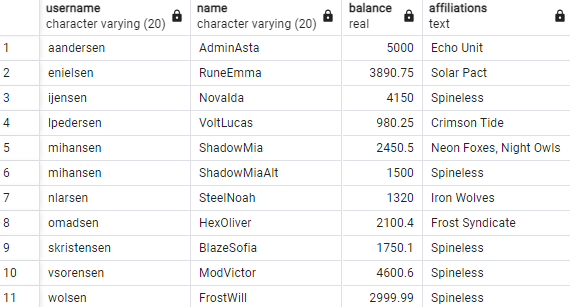
\includegraphics{images/frontpage/View-v_character_overview.png}
\caption{v\_character\_overview}
\end{figure}

This structure provides a clear and compact overview suitable for
application use, administration, and reporting.

\hypertarget{gang-overview-view}{%
\paragraph{Gang Overview View}\label{gang-overview-view}}

The v\_gang\_overview view provides a summarized overview of each gang
and its members.

\begin{Shaded}
\begin{Highlighting}[]
\KeywordTok{CREATE} \KeywordTok{OR} \KeywordTok{REPLACE} \KeywordTok{VIEW}\NormalTok{ v\_gang\_overview }\KeywordTok{AS}
\KeywordTok{SELECT}
\NormalTok{    gangs.name }\KeywordTok{AS}\NormalTok{ gang\_name,}
    \FunctionTok{COALESCE}\NormalTok{(STRING\_AGG(characters.name, }\StringTok{\textquotesingle{}, \textquotesingle{}}\NormalTok{), }\StringTok{\textquotesingle{}No members\textquotesingle{}}\NormalTok{) }\KeywordTok{AS}\NormalTok{ members}
\KeywordTok{FROM}\NormalTok{ gangs}
\KeywordTok{LEFT} \KeywordTok{JOIN}\NormalTok{ gang\_affiliations }\KeywordTok{ON}\NormalTok{ gang\_affiliations.gang\_id }\OperatorTok{=}\NormalTok{ gangs.}\KeywordTok{id}
\KeywordTok{LEFT} \KeywordTok{JOIN}\NormalTok{ characters }\KeywordTok{ON}\NormalTok{ characters.}\KeywordTok{id} \OperatorTok{=}\NormalTok{ gang\_affiliations.character\_id}
\KeywordTok{GROUP} \KeywordTok{BY}\NormalTok{ gangs.name;}
\end{Highlighting}
\end{Shaded}

\textbf{Result}

When querying the view:\\
\texttt{SELECT\ *\ FROM\ v\_gang\_overview;}

\begin{figure}
\centering
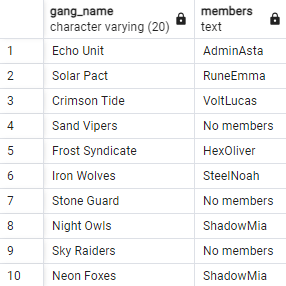
\includegraphics{images/frontpage/View-v_gang_overview.png}
\caption{v\_character\_overview}
\end{figure}

The view combines data from the \texttt{gangs},
\texttt{gang\_affiliations}, and \texttt{characters} tables to present
gang information in a simplified format.

\hypertarget{character-appearance-overview-view}{%
\paragraph{Character Appearance Overview
View}\label{character-appearance-overview-view}}

The v\_character\_appearance view provides a structured overview of each
character's physical attributes

\begin{Shaded}
\begin{Highlighting}[]
\KeywordTok{CREATE} \KeywordTok{OR} \KeywordTok{REPLACE} \KeywordTok{VIEW}\NormalTok{ v\_character\_appearance }\KeywordTok{AS}
\KeywordTok{SELECT}
\NormalTok{    characters.name }\KeywordTok{AS}\NormalTok{ character\_name,}
\NormalTok{    characters.balance }\KeywordTok{AS}\NormalTok{ balance,}
\NormalTok{    genders.name }\KeywordTok{AS}\NormalTok{ gender,}
\NormalTok{    weights.name }\KeywordTok{AS}\NormalTok{ weight,}
\NormalTok{    heights.name }\KeywordTok{AS}\NormalTok{ height,}
\NormalTok{    eyecolors.name }\KeywordTok{AS}\NormalTok{ eye\_color,}
\NormalTok{    skincolors.name }\KeywordTok{AS}\NormalTok{ skin\_color}
\KeywordTok{FROM}\NormalTok{ characters}
\KeywordTok{JOIN}\NormalTok{ genders }\KeywordTok{ON}\NormalTok{ genders.}\KeywordTok{id} \OperatorTok{=}\NormalTok{ characters.gender\_id}
\KeywordTok{JOIN}\NormalTok{ weights }\KeywordTok{ON}\NormalTok{ weights.}\KeywordTok{id} \OperatorTok{=}\NormalTok{ characters.weight\_id}
\KeywordTok{JOIN}\NormalTok{ heights }\KeywordTok{ON}\NormalTok{ heights.}\KeywordTok{id} \OperatorTok{=}\NormalTok{ characters.height\_id}
\KeywordTok{JOIN}\NormalTok{ eyecolors }\KeywordTok{ON}\NormalTok{ eyecolors.}\KeywordTok{id} \OperatorTok{=}\NormalTok{ characters.eyecolor\_id}
\KeywordTok{JOIN}\NormalTok{ skincolors }\KeywordTok{ON}\NormalTok{ skincolors.}\KeywordTok{id} \OperatorTok{=}\NormalTok{ characters.skincolor\_id;}
\end{Highlighting}
\end{Shaded}

Each of these attributes is stored as a foreign key in the
\texttt{characters} table and linked to a corresponding lookup table. By
using joins, the view replaces internal identifier values with readable
attribute names. This makes the data easier to understand and use in
application features, administration, and reporting.

\textbf{Result}

When querying the view:
\texttt{SELECT\ *\ FROM\ v\_character\_appearance;}

\begin{figure}
\centering
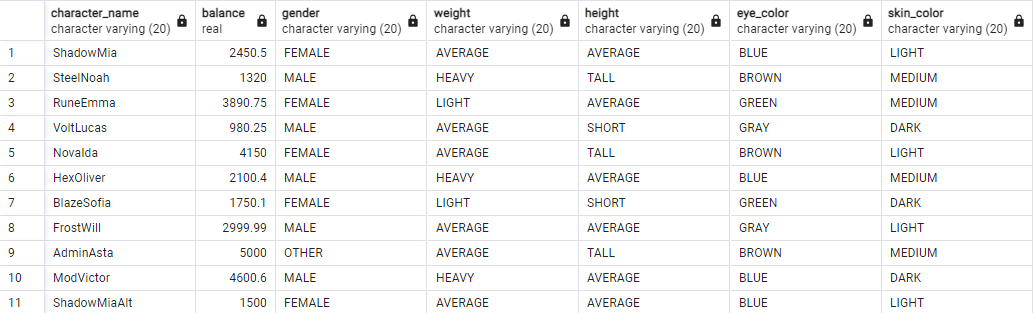
\includegraphics{images/frontpage/View-v_character_appearance.png}
\caption{v\_character\_overview}
\end{figure}

The view simplifies queries by collecting all appearance-related
information in a single logical structure and supports the normalized
database design by keeping descriptive values in dedicated reference
tables.

\hypertarget{triggers}{%
\subsubsection{2.4.2. Triggers}\label{triggers}}

A trigger is a piece of sql code that automatically executes in response
to certain events on a particular table. A trigger can be set to execute
either before or after an insert, update, or delete operation. Triggers
are commonly used to enforce complex business rules, maintain data
integrity, or perform automatic updates based on changes in the
database.

\hypertarget{purpose-of-trigger-in-this-project}{%
\subsubsection{Purpose of trigger in this
project}\label{purpose-of-trigger-in-this-project}}

In this project, a trigger is linked to the characters table. The
purpose of the trigger is to automatically react whenever a new
character is created.

Character creation is a core operation in our RPG game. Each time a new
character is inserted into the database, the system should generate a
message indicating that the character has been successfully created.
Rather than implementing this behavior solely in application code, it is
defined directly in PostgreSQL. This guarantees that the behavior is
executed consistently, even if data insertion occurs from administrative
scripts, test environments, or other services.

\hypertarget{trigger-implementation}{%
\subsubsection{Trigger Implementation}\label{trigger-implementation}}

The trigger is defined as an AFTER INSERT trigger on the characters
table and executes once per inserted row (FOR EACH ROW). When a new
character is inserted, PostgreSQL invokes the trigger function and
exposes the inserted row through the special record variable NEW.

The trigger function uses RAISE NOTICE to send a notice containing the
newly created character's name. Because the trigger runs after the
insert operation, referential integrity is guaranteed at the time the
message is produced.

The trigger looks like this:

\begin{Shaded}
\begin{Highlighting}[]
\KeywordTok{CREATE} \KeywordTok{OR} \KeywordTok{REPLACE} \KeywordTok{FUNCTION}\NormalTok{ fn\_character\_notice()}
\NormalTok{RETURNS }\KeywordTok{trigger}
\NormalTok{LANGUAGE plpgsql}
\KeywordTok{AS}\NormalTok{ $$}
\ControlFlowTok{BEGIN}
\NormalTok{  RAISE NOTICE }\StringTok{\textquotesingle{}Welcome! Your new character created: name=\%\textquotesingle{}}\NormalTok{, }\KeywordTok{NEW}\NormalTok{.name;}
\KeywordTok{RETURN} \KeywordTok{NEW}\NormalTok{;}
\ControlFlowTok{END}\NormalTok{;}
\NormalTok{$$;}

\KeywordTok{DROP} \KeywordTok{TRIGGER} \ControlFlowTok{IF} \KeywordTok{EXISTS}\NormalTok{ trg\_character\_notice }\KeywordTok{ON}\NormalTok{ characters;}

\KeywordTok{CREATE} \KeywordTok{TRIGGER}\NormalTok{ trg\_character\_notice}
    \KeywordTok{AFTER} \KeywordTok{INSERT} \KeywordTok{ON}\NormalTok{ characters}
    \ControlFlowTok{FOR} \KeywordTok{EACH} \KeywordTok{ROW}
    \KeywordTok{EXECUTE} \KeywordTok{FUNCTION}\NormalTok{ fn\_character\_notice();}
\end{Highlighting}
\end{Shaded}

The message is not stored in a database table. Instead, it is sent as a
notice to the client application that performed the insert. This allows
for real-time feedback without modifying the data model or adding extra
tables for logging.

\hypertarget{design-considerations}{%
\subsubsection{Design considerations}\label{design-considerations}}

Using a trigger for this purpose has both advantages and disadvantages:

\begin{itemize}
\tightlist
\item
  \textbf{Advantages}:

  \begin{itemize}
  \tightlist
  \item
    Ensures consistent behavior regardless of how data is inserted.
  \item
    Centralizes the logic in the database, reducing reliance on
    application code.
  \item
    Provides immediate feedback to users or administrators when
    characters are created.
  \end{itemize}
\item
  \textbf{Disadvantages}:

  \begin{itemize}
  \tightlist
  \item
    Reduces transparency of system control flow.
  \item
    Debugging may require inspecting database-level logic.
  \item
    The message is not stored for later retrieval.
  \end{itemize}
\end{itemize}

Given the limited scope of the project, this approach provides a clear
demonstration of automated database behavior without introducing
additional complexity.

\hypertarget{events}{%
\subsubsection{Events}\label{events}}

An event is a piece of SQL code that is scheduled to execute at a
specific time or interval. Events are commonly used for tasks such as
periodic data cleanup, scheduled reporting, or automated maintenance. As
we are using Postgres in this project, we do not have access to
scheduled events. So instead we will show an example of how it would be
done in MySQL.

\hypertarget{purpose-of-event-in-this-project}{%
\subsubsection{Purpose of event in this
project}\label{purpose-of-event-in-this-project}}

Our thought was that we would use a weekly scheduled event to announce
the richest person in our game. The event would run every week and
execute a query to find the character with the highest balance. Then it
would raise notice with the name of the richest character and their
balance. We thought about creating a Notification table to store the
results of the event, but we decided to keep it simple and just use
RAISE NOTICE for demonstration purposes.

\hypertarget{event-implementation}{%
\subsubsection{Event Implementation}\label{event-implementation}}

\begin{Shaded}
\begin{Highlighting}[]

\end{Highlighting}
\end{Shaded}

\hypertarget{decision-not-made-yet.-work-in-progress}{%
\subsubsection{decision not made yet. work in
progress}\label{decision-not-made-yet.-work-in-progress}}

\hypertarget{design-considerations-1}{%
\subsubsection{Design considerations}\label{design-considerations-1}}

Using an event for this purpose has both advantages and disadvantages:

\begin{itemize}
\tightlist
\item
  \textbf{Advantages}:

  \begin{itemize}
  \tightlist
  \item
    Automates regular tasks without manual intervention.
  \item
    Provides timely updates to users or administrators.
  \item
    Can be used for a wide range of scheduled operations.
  \end{itemize}
\item
  \textbf{Disadvantages}:

  \begin{itemize}
  \tightlist
  \item
    May require additional setup and configuration in the database.
  \item
    Debugging scheduled events can be more complex than triggers.
  \item
    The output may not be easily accessible if not stored in a table.
  \end{itemize}
\end{itemize}

\hypertarget{events-1}{%
\subsubsection{2.4.3. Events}\label{events-1}}

\hypertarget{introduction-1}{%
\paragraph{Introduction}\label{introduction-1}}

In many relational database courses, ``events'' usually means scheduled
database tasks that run automatically at fixed times. PostgreSQL does
not provide a built-in \texttt{CREATE\ EVENT} feature like MySQL. For
this reason, this project implements scheduled behavior using a
cron-based approach instead.

The implementation is placed in \texttt{sqls/daily\_loyalty\_bonus.sql}.

\hypertarget{why-cron-jobs-in-postgresql}{%
\paragraph{Why cron jobs in
PostgreSQL}\label{why-cron-jobs-in-postgresql}}

Because PostgreSQL has no native event scheduler syntax, we use the
\texttt{pg\_cron} extension to execute SQL commands on a defined
schedule. This gives us event-like behavior while staying inside
PostgreSQL.

In this project, the scheduled task runs every day at \textbf{00:01} and
updates each character's balance according to gang membership rules:

\begin{itemize}
\tightlist
\item
  Characters with gang affiliation receive a loyalty bonus.
\item
  Characters without gang affiliation receive a fixed fallback bonus of
  \texttt{100}.
\end{itemize}

\hypertarget{cron-job-file-walkthrough}{%
\paragraph{Cron job file walkthrough}\label{cron-job-file-walkthrough}}

The full implementation is in \texttt{sqls/daily\_loyalty\_bonus.sql}
and is structured in three parts:

\begin{enumerate}
\def\labelenumi{\arabic{enumi}.}
\tightlist
\item
  Enable extension:
\end{enumerate}

\begin{Shaded}
\begin{Highlighting}[]
\KeywordTok{CREATE}\NormalTok{ EXTENSION }\ControlFlowTok{IF} \KeywordTok{NOT} \KeywordTok{EXISTS}\NormalTok{ pg\_cron;}
\end{Highlighting}
\end{Shaded}

This ensures cron scheduling is available in the current database.

\begin{enumerate}
\def\labelenumi{\arabic{enumi}.}
\setcounter{enumi}{1}
\tightlist
\item
  Replace existing job with same name:
\end{enumerate}

\begin{Shaded}
\begin{Highlighting}[]
\NormalTok{DO $$}
\KeywordTok{DECLARE}
\NormalTok{    v\_job\_id }\DataTypeTok{integer}\NormalTok{;}
\ControlFlowTok{BEGIN}
    \KeywordTok{SELECT}\NormalTok{ jobid}
    \KeywordTok{INTO}\NormalTok{ v\_job\_id}
    \KeywordTok{FROM}\NormalTok{ cron.job}
    \KeywordTok{WHERE}\NormalTok{ jobname }\OperatorTok{=} \StringTok{\textquotesingle{}daily\_loyalty\_bonus\textquotesingle{}}\NormalTok{;}

    \ControlFlowTok{IF}\NormalTok{ v\_job\_id }\KeywordTok{IS} \KeywordTok{NOT} \KeywordTok{NULL} \ControlFlowTok{THEN}
\NormalTok{        PERFORM cron.unschedule(v\_job\_id);}
    \ControlFlowTok{END} \ControlFlowTok{IF}\NormalTok{;}
\ControlFlowTok{END}\NormalTok{ $$;}
\end{Highlighting}
\end{Shaded}

This prevents duplicate schedules if the script is executed multiple
times.

\begin{enumerate}
\def\labelenumi{\arabic{enumi}.}
\setcounter{enumi}{2}
\tightlist
\item
  Schedule daily payout at \texttt{00:01}:
\end{enumerate}

\begin{Shaded}
\begin{Highlighting}[]
\KeywordTok{SELECT}\NormalTok{ cron.schedule(}
    \StringTok{\textquotesingle{}daily\_loyalty\_bonus\textquotesingle{}}\NormalTok{,}
    \StringTok{\textquotesingle{}1 0 * * *\textquotesingle{}}\NormalTok{,}
\NormalTok{    $cron$}
    \KeywordTok{UPDATE}\NormalTok{ characters c}
    \KeywordTok{SET}\NormalTok{ balance }\OperatorTok{=}\NormalTok{ c.balance }\OperatorTok{+} \FunctionTok{COALESCE}\NormalTok{(b.bonus, }\DecValTok{100}\NormalTok{)}
    \KeywordTok{FROM}\NormalTok{ (}
        \KeywordTok{SELECT}
\NormalTok{            c2.}\KeywordTok{id} \KeywordTok{AS}\NormalTok{ character\_id,}
            \FunctionTok{SUM}\NormalTok{(}\FunctionTok{GREATEST}\NormalTok{((}\FunctionTok{CURRENT\_DATE} \OperatorTok{{-}}\NormalTok{ ga.join\_date), }\DecValTok{0}\NormalTok{)):}\CharTok{:double} \DataTypeTok{precision} \KeywordTok{AS}\NormalTok{ bonus}
        \KeywordTok{FROM}\NormalTok{ characters c2}
        \KeywordTok{LEFT} \KeywordTok{JOIN}\NormalTok{ gang\_affiliations ga}
            \KeywordTok{ON}\NormalTok{ ga.character\_id }\OperatorTok{=}\NormalTok{ c2.}\KeywordTok{id}
        \KeywordTok{GROUP} \KeywordTok{BY}\NormalTok{ c2.}\KeywordTok{id}
\NormalTok{    ) b}
    \KeywordTok{WHERE}\NormalTok{ c.}\KeywordTok{id} \OperatorTok{=}\NormalTok{ b.character\_id;}
\NormalTok{    $cron$}
\NormalTok{);}
\end{Highlighting}
\end{Shaded}

How this works:

\begin{itemize}
\tightlist
\item
  \texttt{\textquotesingle{}1\ 0\ *\ *\ *\textquotesingle{}} means every
  day at 00:01.
\item
  \texttt{LEFT\ JOIN} keeps all characters in scope, even without gang
  rows.
\item
  \texttt{CURRENT\_DATE\ -\ ga.join\_date} calculates number of days in
  gang.
\item
  \texttt{SUM(...)} adds bonus days if a character has multiple
  affiliations.
\item
  \texttt{COALESCE(b.bonus,\ 100)} applies fallback \texttt{100} when no
  gang bonus is available.
\end{itemize}

\hypertarget{summary}{%
\paragraph{Summary}\label{summary}}

PostgreSQL does not have native event objects, so scheduled automation
is implemented using cron jobs. In this project, the daily loyalty
payout is implemented as a reusable SQL script in
\texttt{sqls/daily\_loyalty\_bonus.sql}, providing predictable and fully
database-side automation.

\newpage

\hypertarget{realistic-data}{%
\subsection{2.5. Realistic data}\label{realistic-data}}

\hypertarget{introduction-2}{%
\subsubsection{Introduction}\label{introduction-2}}

The project includes a dedicated seed script, \texttt{sqls/seed.sql},
that creates a realistic baseline dataset for demos, testing, and
validation. Instead of random values, the script inserts coherent player
profiles, characters, houses, and gang memberships, so queries return
believable results and relationship rules can be verified in practice.

\hypertarget{script-structure}{%
\subsubsection{Script Structure}\label{script-structure}}

The script starts by opening a transaction and resetting all relevant
tables. This makes each run deterministic and easy to repeat.

In this context, \emph{deterministic} means that the script produces the
same data state every time it is executed on the same schema.

\begin{Shaded}
\begin{Highlighting}[]
\ControlFlowTok{BEGIN}\NormalTok{;}
\KeywordTok{TRUNCATE} \KeywordTok{TABLE}
\NormalTok{    gang\_affiliations,}
\NormalTok{    characters,}
\NormalTok{    profiles,}
\NormalTok{    gangs,}
\NormalTok{    houses,}
    \KeywordTok{roles}\NormalTok{,}
\NormalTok{    genders,}
\NormalTok{    weights,}
\NormalTok{    heights,}
\NormalTok{    eyecolors,}
\NormalTok{    skincolors}
\NormalTok{RESTART IDENTITY }\KeywordTok{CASCADE}\NormalTok{;}
\end{Highlighting}
\end{Shaded}

\texttt{TRUNCATE} removes all rows from the listed tables very quickly.
\texttt{RESTART\ IDENTITY} resets auto-increment IDs back to their
starting values, and \texttt{CASCADE} ensures dependent tables are also
cleared safely.

After reset, the script inserts stable reference data first, followed by
gangs and player profiles.

\begin{Shaded}
\begin{Highlighting}[]
\KeywordTok{INSERT} \KeywordTok{INTO} \KeywordTok{roles}\NormalTok{ (}\KeywordTok{id}\NormalTok{, name) }\KeywordTok{VALUES}\NormalTok{ (}\DecValTok{1}\NormalTok{, }\StringTok{\textquotesingle{}USER\textquotesingle{}}\NormalTok{), (}\DecValTok{2}\NormalTok{, }\StringTok{\textquotesingle{}ADMIN\textquotesingle{}}\NormalTok{);}
\KeywordTok{INSERT} \KeywordTok{INTO}\NormalTok{ genders (}\KeywordTok{id}\NormalTok{, name) }\KeywordTok{VALUES}\NormalTok{ (}\DecValTok{1}\NormalTok{, }\StringTok{\textquotesingle{}MALE\textquotesingle{}}\NormalTok{), (}\DecValTok{2}\NormalTok{, }\StringTok{\textquotesingle{}FEMALE\textquotesingle{}}\NormalTok{), (}\DecValTok{3}\NormalTok{, }\StringTok{\textquotesingle{}OTHER\textquotesingle{}}\NormalTok{);}
\KeywordTok{INSERT} \KeywordTok{INTO}\NormalTok{ weights (}\KeywordTok{id}\NormalTok{, name) }\KeywordTok{VALUES}\NormalTok{ (}\DecValTok{1}\NormalTok{, }\StringTok{\textquotesingle{}LIGHT\textquotesingle{}}\NormalTok{), (}\DecValTok{2}\NormalTok{, }\StringTok{\textquotesingle{}AVERAGE\textquotesingle{}}\NormalTok{), (}\DecValTok{3}\NormalTok{, }\StringTok{\textquotesingle{}HEAVY\textquotesingle{}}\NormalTok{);}
\KeywordTok{INSERT} \KeywordTok{INTO}\NormalTok{ heights (}\KeywordTok{id}\NormalTok{, name) }\KeywordTok{VALUES}\NormalTok{ (}\DecValTok{1}\NormalTok{, }\StringTok{\textquotesingle{}SHORT\textquotesingle{}}\NormalTok{), (}\DecValTok{2}\NormalTok{, }\StringTok{\textquotesingle{}AVERAGE\textquotesingle{}}\NormalTok{), (}\DecValTok{3}\NormalTok{, }\StringTok{\textquotesingle{}TALL\textquotesingle{}}\NormalTok{);}
\end{Highlighting}
\end{Shaded}

\hypertarget{schema-aware-character-and-house-seeding}{%
\subsubsection{Schema-aware character and house
seeding}\label{schema-aware-character-and-house-seeding}}

To support schema variants, seeding for \texttt{characters} and
\texttt{houses} is handled in a \texttt{DO} block. It checks where the
foreign key is placed and inserts in the correct order to avoid
referential errors.

\begin{Shaded}
\begin{Highlighting}[]
\ControlFlowTok{IF}\NormalTok{ characters\_has\_house\_id }\KeywordTok{AND} \KeywordTok{NOT}\NormalTok{ houses\_has\_character\_id }\ControlFlowTok{THEN}
    \KeywordTok{INSERT} \KeywordTok{INTO}\NormalTok{ houses (}\KeywordTok{id}\NormalTok{, amount\_rooms, amount\_bathrooms) }\KeywordTok{VALUES}
\NormalTok{        (}\DecValTok{1}\NormalTok{, }\DecValTok{2}\NormalTok{, }\DecValTok{1}\NormalTok{), (}\DecValTok{2}\NormalTok{, }\DecValTok{3}\NormalTok{, }\DecValTok{2}\NormalTok{), (}\DecValTok{3}\NormalTok{, }\DecValTok{1}\NormalTok{, }\DecValTok{1}\NormalTok{);}

    \KeywordTok{INSERT} \KeywordTok{INTO}\NormalTok{ characters (}
        \KeywordTok{id}\NormalTok{, name, balance, profile\_id, gender\_id, skincolor\_id,}
\NormalTok{        eyecolor\_id, height\_id, weight\_id, house\_id}
\NormalTok{    ) }\KeywordTok{VALUES}
\NormalTok{        (}\DecValTok{1}\NormalTok{, }\StringTok{\textquotesingle{}ShadowMia\textquotesingle{}}\NormalTok{, }\FloatTok{2450.50}\NormalTok{, }\DecValTok{1}\NormalTok{, }\DecValTok{2}\NormalTok{, }\DecValTok{1}\NormalTok{, }\DecValTok{2}\NormalTok{, }\DecValTok{2}\NormalTok{, }\DecValTok{2}\NormalTok{, }\DecValTok{1}\NormalTok{),}
\NormalTok{        (}\DecValTok{2}\NormalTok{, }\StringTok{\textquotesingle{}SteelNoah\textquotesingle{}}\NormalTok{, }\FloatTok{1320.00}\NormalTok{, }\DecValTok{2}\NormalTok{, }\DecValTok{1}\NormalTok{, }\DecValTok{2}\NormalTok{, }\DecValTok{1}\NormalTok{, }\DecValTok{3}\NormalTok{, }\DecValTok{3}\NormalTok{, }\DecValTok{2}\NormalTok{);}
\ControlFlowTok{END} \ControlFlowTok{IF}\NormalTok{;}
\end{Highlighting}
\end{Shaded}

The condition means: if \texttt{characters} contains \texttt{house\_id}
and \texttt{houses} does not contain \texttt{character\_id}, then the
foreign key points from \texttt{characters} to \texttt{houses}. In that
case, \texttt{houses} must be inserted first.

For
\texttt{INSERT\ INTO\ houses\ (id,\ amount\_rooms,\ amount\_bathrooms)},
each tuple follows that exact column order:

\begin{itemize}
\tightlist
\item
  \texttt{(1,\ 2,\ 1)} = \texttt{id\ =\ 1},
  \texttt{amount\_rooms\ =\ 2}, \texttt{amount\_bathrooms\ =\ 1}
\item
  \texttt{(2,\ 3,\ 2)} = \texttt{id\ =\ 2},
  \texttt{amount\_rooms\ =\ 3}, \texttt{amount\_bathrooms\ =\ 2}
\item
  \texttt{(3,\ 1,\ 1)} = \texttt{id\ =\ 3},
  \texttt{amount\_rooms\ =\ 1}, \texttt{amount\_bathrooms\ =\ 1}
\end{itemize}

\hypertarget{gang-membership-data}{%
\subsubsection{Gang membership data}\label{gang-membership-data}}

Gang membership is optional in the model, so only a subset of characters
receives rows in \texttt{gang\_affiliations}. This intentionally
demonstrates both valid states: characters with gang membership and
characters without gang membership.

\begin{Shaded}
\begin{Highlighting}[]
\KeywordTok{INSERT} \KeywordTok{INTO}\NormalTok{ gang\_affiliations (character\_id, gang\_id, join\_date) }\KeywordTok{VALUES}
\NormalTok{    (}\DecValTok{1}\NormalTok{, }\DecValTok{2}\NormalTok{, }\StringTok{\textquotesingle{}2025{-}01{-}12\textquotesingle{}}\NormalTok{),}
\NormalTok{    (}\DecValTok{2}\NormalTok{, }\DecValTok{1}\NormalTok{, }\StringTok{\textquotesingle{}2025{-}02{-}03\textquotesingle{}}\NormalTok{),}
\NormalTok{    (}\DecValTok{3}\NormalTok{, }\DecValTok{7}\NormalTok{, }\StringTok{\textquotesingle{}2025{-}03{-}22\textquotesingle{}}\NormalTok{),}
\NormalTok{    (}\DecValTok{4}\NormalTok{, }\DecValTok{5}\NormalTok{, }\StringTok{\textquotesingle{}2025{-}04{-}10\textquotesingle{}}\NormalTok{);}
\end{Highlighting}
\end{Shaded}

Finally, all inserts are persisted in one atomic commit.

\begin{Shaded}
\begin{Highlighting}[]
\KeywordTok{COMMIT}\NormalTok{;}
\end{Highlighting}
\end{Shaded}

\hypertarget{security-and-access-control}{%
\subsection{2.6. Security and access
control}\label{security-and-access-control}}

\hypertarget{explanation-of-users-and-privileges}{%
\subsubsection{2.6.1. Explanation of users and
privileges}\label{explanation-of-users-and-privileges}}

Database access should follow least-privilege principles, so each role
gets only the permissions required for its tasks. A typical split is:

\begin{itemize}
\tightlist
\item
  \texttt{app\_user}: runtime role for the Java application
  (\texttt{SELECT}, \texttt{INSERT}, \texttt{UPDATE}, \texttt{DELETE} on
  business tables).
\item
  \texttt{report\_user}: read-only role for analytics and reporting
  (\texttt{SELECT} only, especially on views).
\item
  \texttt{admin\_user}: migration and maintenance role (\texttt{CREATE},
  \texttt{ALTER}, \texttt{DROP}, and role management).
\end{itemize}

Example grants:

\begin{Shaded}
\begin{Highlighting}[]
\KeywordTok{CREATE} \KeywordTok{ROLE}\NormalTok{ app\_user LOGIN }\KeywordTok{PASSWORD} \StringTok{\textquotesingle{}change\_me\textquotesingle{}}\NormalTok{;}
\KeywordTok{CREATE} \KeywordTok{ROLE}\NormalTok{ report\_user LOGIN }\KeywordTok{PASSWORD} \StringTok{\textquotesingle{}change\_me\textquotesingle{}}\NormalTok{;}

\KeywordTok{GRANT} \KeywordTok{USAGE} \KeywordTok{ON} \KeywordTok{SCHEMA} \KeywordTok{public} \KeywordTok{TO}\NormalTok{ app\_user, report\_user;}
\KeywordTok{GRANT} \KeywordTok{SELECT}\NormalTok{, }\KeywordTok{INSERT}\NormalTok{, }\KeywordTok{UPDATE}\NormalTok{, }\KeywordTok{DELETE} \KeywordTok{ON} \KeywordTok{ALL} \KeywordTok{TABLES} \KeywordTok{IN} \KeywordTok{SCHEMA} \KeywordTok{public} \KeywordTok{TO}\NormalTok{ app\_user;}
\KeywordTok{GRANT} \KeywordTok{SELECT} \KeywordTok{ON}\NormalTok{ v\_character\_overview, v\_gang\_overview, v\_character\_appearance }\KeywordTok{TO}\NormalTok{ report\_user;}
\end{Highlighting}
\end{Shaded}

This model prevents accidental schema changes from application accounts
and limits exposure of sensitive data to only what each user type needs.

\hypertarget{chapter-summary}{%
\subsection{2.7. Chapter summary}\label{chapter-summary}}

This chapter moved from requirements to implementation in a single
traceable line:

\begin{itemize}
\tightlist
\item
  business rules were defined,
\item
  relationships were modeled and normalized,
\item
  schema execution and integrity constraints were documented,
\item
  views/triggers/events were explained as stored objects,
\item
  realistic seed data and privilege strategy completed the operational
  setup.
\end{itemize}

Together, these elements make the database understandable, reproducible,
and ready for both development and deployment.

\newpage

\hypertarget{appendix-a.-links-and-file-references}{%
\subsection{Appendix A. Links and file
references}\label{appendix-a.-links-and-file-references}}

\hypertarget{external-links-references}{%
\subsubsection{External links
(references)}\label{external-links-references}}

\begin{itemize}
\tightlist
\item
  https://www.postgresql.org/docs/
\item
  https://docs.oracle.com/en/java/javase/17/
\item
  https://maven.apache.org/guides/
\item
  https://hibernate.org/orm/documentation/
\end{itemize}

\hypertarget{file-references-used-in-report}{%
\subsubsection{File references used in
report}\label{file-references-used-in-report}}

\begin{itemize}
\tightlist
\item
  docker-compose.yml
\item
  sqls/schema.sql
\item
  sqls/daily\_loyalty\_bonus.sql
\item
  sqls/seed.sql
\item
  images/frontpage/Document3.png
\item
  images/frontpage/Graph-Database.png
\item
  images/frontpage/what-is-a-relational-database.jpg
\item
  images/conceptual-logical-physical/conceptual-model-2026-02-10.png
\item
  images/conceptual-logical-physical/logical-model-2026-02-10.png
\item
  images/conceptual-logical-physical/physical-model-2026-02-10.png
\item
  images/frontpage/View-v\_character\_overview.png
\item
  images/frontpage/View-v\_gang\_overview.png
\item
  images/frontpage/View-v\_character\_appearance.png
\end{itemize}
